\documentclass[12pt,a4paper]{article}
\usepackage{graphicx}
\usepackage{amsmath}
\usepackage{amssymb}
\usepackage{subfigure}
\usepackage{booktabs}
\usepackage{color}
\usepackage{listings}
\usepackage{eurosym}
\usepackage{mathtools} % for \mydef
\usepackage{float}
\usepackage{natbib}
\usepackage{gensymb} % for \degree
%\usepackage{authblk} % for multiple authors with different affiliations
\usepackage[small]{titlesec}
\usepackage[displaymath, mathlines]{lineno}

% see http://tex.stackexchange.com/questions/99316/symbol-for-external-links
\usepackage{fontawesome}
\usepackage[hidelinks]{hyperref}
% Redefinition, symbol included in link:
\let\orighref\href
\renewcommand{\href}[2]{\underline{\orighref{#1}{#2}}}
% hyphens option for hyperref: enables line-breaks at hyphens. Otherwise only at slashes /. Ugly
%\PassOptionsToPackage{hyphens}{url}\usepackage{hyperref}

\addtolength{\oddsidemargin}{-2cm}
\addtolength{\evensidemargin}{-2cm}
\addtolength{\textwidth}{4cm}
\addtolength{\topmargin}{-2cm}
\addtolength{\textheight}{2cm}

%%%%%%%%%%%%%%%%%%%%%%%%%%%%%%%%%%%%%%%%%%%%%%%%
% REMOVE FOR FINAL VERSION


%%DRAFT HEADERS on normal pages
%\usepackage{fancyhdr}
%\pagestyle{fancy}
%\fancyhf{} % clear all headers and footers
%\fancyhead[C]{{\bf DRAFT}}
%\cfoot{\thepage}
%%DRAFT HEADERS on TOC and Chapter pages
%\fancypagestyle{plain}{
%	\fancyhf{}
%	\fancyhead[C]{{\bf DRAFT}}
%	\cfoot{\thepage}
%}
%%DRAFT HEADERS on title pages
%\fancypagestyle{empty}{
%	\fancyhf{}
%	\fancyhead[C]{{\bf DRAFT}}
%}

%%%%%%%%%%%%%%%%%%%%%%%%%%%%%%%%%%%%%%%%%%%%%%%%%%%%%%%%


\renewcommand{\familydefault}{\sfdefault}

\graphicspath{{figures/}{matlab/omega/figures/}} 

%\linenumbers

\title{
	{\bf DRAFT}\\
	Notes on running ROMS on Amazon Web Services 
}

\author{Stefan Riha\thanks{Email: stefan@sriha.net}}
%\date{}

\begin{document}
	\setlength{\parindent}{0cm}
	\maketitle

\section{Preliminary results}
	All results shown were produced with ROMS \citep{shchepetkin2005regional}, compiled with Open MPI using gfortran.
	
	\begin{figure}[H]
		\centering
		\includegraphics[width=0.5\textwidth]{met_t2micro.pdf}
		\caption{Time (in seconds) spent per process for the ROMS "small" benchmark test (benchmark1.in), as function of the number of processes. Computations are performed on t2.micro instances of AWS, which have one vCPU per (virtual) node (2016/11/01). Each data point shows the average over all processes, measured from one single experiment. The inset shows the domain partition (tiling) of the 512x64(x30) point domain. The result suggests that partitioning along the first dimension yields better performance, and that the problem scales nonlinearly.}
		\label{fig:met_t2micro}
	\end{figure}

	\begin{figure}[H]
	\centering
	\includegraphics[width=0.5\textwidth]{met_c4large.pdf}
	\caption{Same as Fig. \ref{fig:met_t2micro}, but computations are performed on c4.large instances of AWS, which have 2 vCPUs per (virtual) node. In the case of c4 instances, a vCPU is defined as a single thread of a custom 2.9 GHz Intel Xeon E5-2666 v3 (Haswell) processor (2016/11/01).}
	\label{fig:met_c4large}
\end{figure}

\begin{figure}[H]
	\centering
	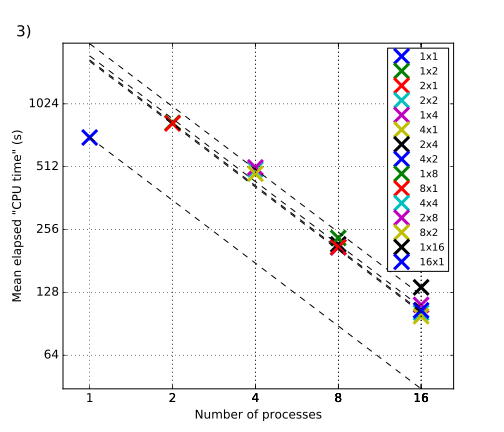
\includegraphics[width=0.5\textwidth]{met_c44xlarge.pdf}
	\caption{Time (in seconds) spent per process for the ROMS "medium" benchmark test (benchmark2.in), as function of the number of processes. Computations are performed on c4.4xlarge instances of AWS, which have 16 vCPUs per (virtual) node.}
	\label{fig:met_c4large}
\end{figure}
	
\bibliography{main.bib}
\bibliographystyle{model2-names}

\end{document}

 
